\begin{center}
\fbox{\fbox{\parbox{6.5in}{\centering
\begin{flushleft}

\vspace{2mm}
\hspace{5mm}
\textbf{\underline{Silinder}}

\vspace{2mm}
\hspace{5mm}
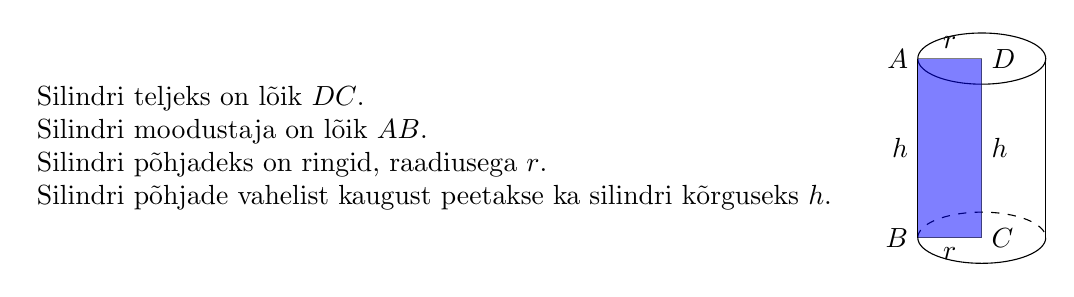
\begin{tikzpicture}[scale=0.65]
\draw (0,0) ellipse (1.25 and 0.5);
\draw (-1.25,0) -- (-1.25,-3.5);
\draw (-1.25,-3.5) arc (180:360:1.25 and 0.5);
\draw [dashed] (-1.25,-3.5) arc (180:360:1.25 and -0.5);
\draw (1.25,-3.5) -- (1.25,0); 

\draw[fill=blue, opacity=0.5] (-1.25,0)--(0,0)--(0,-3.5)--(-1.25,-3.5);

\node[right] at (0,-1.75){$h$};
\node[left] at (-1.25,-1.75){$h$};
\node[above] at (-0.625,0){$r$};
\node[below] at (-0.625,-3.5){$r$};
\node[left] at (-1.25,0) {$A$};
\node[left] at (-1.25,-3.5){$B$};
\node[right] at (0,-3.5){$C$};
\node[right] at (0,0){$D$};
\node[text width=11cm] at (-10,-1.75){Silindri teljeks on lõik $DC$.\\
Silindri moodustaja on lõik $AB$.\\
Silindri põhjadeks on ringid, raadiusega $r$.\\
Silindri põhjade vahelist kaugust peetakse ka silindri kõrguseks $h$.};
\end{tikzpicture}

\vspace{2mm}
\hspace{5mm}
\textbf{Silindri pindala}

\vspace{2mm}
\hspace{5mm}
Silindri pindala koosneb kahest põhja pinadalast, mis on ringid, ning ühest ristkülikust, mis on saadud\\ \hspace{5mm} silindri külje lõikamisel mööda moodustajat (järelikult selle ristküliku kõrgus on $h$ ja laius põhja\\ \hspace{5mm} ümbermõõt ehk ringjoone pikkus $C$).

\begin{equation}
\label{43_eq1}
\boxed{S_{p}=\pi r^{2}}
\end{equation}

\begin{equation}
\label{43_eq2}
\boxed{S_{k}=C h=2\pi r h}
\end{equation}

\hspace{5mm}
kus $\pi \approx 3.14$, $r$ on ringi raadius, $C$ ringi ümbermõõt, $h$ silindri kõrgus.

\vspace{2mm}
\hspace{5mm}
Ning kuna silindril on kaks põhja, siis täispindala avaldub nii:

\begin{equation}
\label{43_eq3}
\boxed{S_{t}=2S_{p}+S_{k}}
\end{equation}

\vspace{2mm}
\hspace{5mm}
\textbf{Silindri ruumala}

\begin{equation}
\label{43_eq4}
\boxed{V=S_{p}\cdot h}
\end{equation}

\hspace{5mm}
kus $S_{p}$ on silindri põhja pindala, $h$ silindri kõrgus.

\vspace{2mm}
\hspace{5mm}
\textbf{\underline{Koonus}}

\vspace{2mm}
\hspace{5mm}
\begin{tikzpicture}[scale=0.8]
\draw (0,0) -- (-1.25,-3.5);
\draw (-1.25,-3.5) arc (180:360:1.25 and 0.5);
\draw [dashed] (-1.25,-3.5) arc (180:360:1.25 and -0.5);
\draw (1.25,-3.5) -- (0,0); 
\draw[fill=blue, opacity=0.5] (1.25,-3.5)--(0,0)--(0,-3.5)--cycle;

\coordinate (A) at (0,0);
\coordinate (B) at (0,-3.5);
\coordinate (C) at (1.25,-3.5);

\pic [draw, angle radius = 3mm, line width=0.4mm] {angle=C--B--A} node at (0.1,-3.4){$\cdot$};

\path (B)--(C) coordinate[pos=0.5](r);
\path (C)--(A) coordinate[pos=0.5](m);
\path (A)--(B) coordinate[pos=0.5](h);
\node[left] at (h){$h$};
\node[below] at (r){$r$};
\node[right] at (m){$m$};


\node[text width=10cm] at (-10,-1.75) {Koonuse põhjaks on ring, seega põhja pindala on:\\

\begin{equation}
\label{43_eq5}
\boxed{S_{p} = \pi r^{2}}
\end{equation}
\\
Koonuse külgpindala on:

\begin{equation}
\label{43_eq6}
\boxed{S_{k}=\pi r m = \dfrac{Cm}{2}}
\end{equation}};
\end{tikzpicture}

\hspace{5mm}
kus $\pi \approx 3.14$, $r$ on ringi raadius, $m$ on koonuse moodustaja (uuri joonist) ning $C$ on ringjoone pikkus\\ \hspace{5mm} ehk ümbermõõt.

\vspace{2mm}
\hspace{5mm}
Täispindala on järelikult:

\begin{equation}
\label{43_eq7}
\boxed{S_{t}=S_{p}+S_{k}}
\end{equation}

\end{flushleft}
}}}
\end{center}



\pagebreak
\begin{center}
\fbox{\fbox{\parbox{6.5in}{\centering
\begin{flushleft}

\vspace{2mm}
\hspace{5mm}
Koonuse ruumala avaldub aga järgmiselt:
\begin{equation}
\boxed{V=\dfrac{1}{3}S_{p}\cdot h}
\end{equation}

\hspace{5mm}
kus $S_{p}$ on koonuse põhja pindala, $h$ on koonuse kõrgus.

\vspace{2mm}
\hspace{5mm}
\textbf{\underline{Kera}}

\vspace{2mm}
\hspace{5mm}
\begin{tikzpicture}

\draw (-1.25,0) arc (180:360:1.25 and 0.5);
\draw [dashed] (-1.25,0) arc (180:360:1.25 and -0.5);
\draw[fill=blue, opacity=0.5] (0,0) circle (1.25);
\draw[fill=black] (0,0) circle (0.035);
\draw[dashed] (0,0)--(1.25,0);

\path (0,0)--(1.25,0) coordinate[pos=0.5](r);
\node[above] at (r){$R$};

\node[text width=11cm] at (-8,0){ Kera pindala valem:

\begin{equation}
\label{43_eq8}
\boxed{S=4\pi R^{2}}
\end{equation}

\vspace{2mm}
Kera ruumala valem:

\begin{equation}
\label{43_eq9}
\boxed{V=\dfrac{4}{3}\pi R^{3}}
\end{equation}

\vspace{2mm}
kus $\pi \approx 3.14$ ning $R$ on kera raadius.};
\end{tikzpicture}


\end{flushleft}
}}}
\end{center}
\vspace{0.5cm}

\textbf{Märkmed}\\
\vspace{2mm}
\begin{mdframed}[style=graphpaper]
\vspace{12cm}
\end{mdframed}